Precision frontier experiments require very high statistics as well as extensive evaluation of systematic uncertainties, backgrounds, biases and distortions in the data selection criteria. The two experiments, TRIUMF PIENU and PSI PEN  provide highly insightful information on the  limitations of their techniques and the principal systematic effects. We will briefly describe the general characteristics of the decay channels measured as well as discuss the designs adopted by the PIENU and PEN experiments.

The previous measurements were performed using stopped pions that decay at rest either directly to a positron and a neutrino ($\pi^+ \rightarrow e^+ \nu$ decay) or first to a muon (and associated neutrino) that subsequently undergoes 3-body decay at rest in the target (decay chain $\pi^+ \rightarrow \mu^+ \rightarrow e^+$). The  energy and time characteristics of the positrons emerging from those two decays are very different, and thus can be used to distinguish the decay channels. By measuring the ratio of positrons detected from the two channels, many systematic effects (e.g. pion counting, solid angle acceptance, efficiency, etc.) cancel out to first order, aiding in reaching high precision.


Positrons arising from $\pi^+ \rightarrow e^+ \nu$ are monoenergetic giving  69.3 MeV of kinetic energy. The timing distribution is an exponential with the pion lifetime. 
The energy distribution of positrons arising from $\pi^+ \rightarrow \mu^+ \rightarrow e^+$ is the so-called Michel spectrum, extending from 0 to 52.3 MeV of kinetic energy. The timing distribution is the convolution of a pion lifetime and a muon lifetime. Simulated energy and timing distributions for $\pi^+ \to e^+ \nu$ and $\pi^+ \to \mu^+ \to e^+$ events are shown in Fig~\ref{fig:MC_pienu_pimue_time_energy}.

\begin{figure}[h!]
\centering
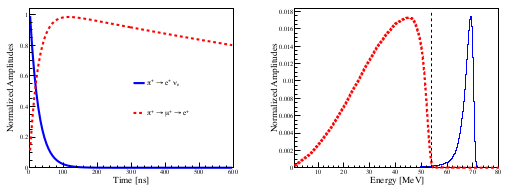
\includegraphics[scale=1.0]{sections/figures/MC_pienu_pimue_time_energy.png}
\caption{Simulated energy (a) and timing (b) distributions for $\pi^+ \to e^+ \nu$ (blue) and $\pi^+ \to \mu^+ \to e^+$ (red) events. }
\label{fig:MC_pienu_pimue_time_energy}
\end{figure}

Since the energy deposited by the decay positrons and their time distributions are important discrimination criteria between the two decay channels,  essential characteristics of the experimental setup  include a high energy resolution calorimeter and fast timing detectors, combined with high frequency, high linearity, signal digitizers.

Muons from  the $\pi^+ \rightarrow \mu^+ \rightarrow e^+$ decay chain deposit $\sim$ 4 MeV in the pion stopping target, which provides an additional handle to discriminate between the two decay modes. The target should thus ideally provide high resolution in energy and cover a large dynamic range to avoid saturation. 
Backgrounds in the time distribution come from decays-in-flight of both pions and muons, necessitating the inclusion of several sets of tracking detectors and a compact detector assembly.

Despite being  mono-energetic the positrons originating from $\pi^+ \rightarrow e^+ \nu$ decays have their energy distribution broadened due to finite energy resolution of the calorimeter, shower leakages of low energy photons from the sides and ends of the calorimeter as well as the presence of radiative decays. Those effects result in a low energy tail hidden under the Michel spectrum and lead to the main correction and largest source of systematic effects in the branching ratio measurement. In order to minimize the energy tail for a precise experiment, a high resolution,  high radiation-length, and high acceptance calorimeter must be chosen.     

%Both experiments used plastic scintillator as the stopping target, and crystal calorimeters for the positron energy measurement. The use of total absorption calorimeters for energy measurements complements the theoretical predictions, which include radiative effects (i.e. $\pi^+ \rightarrow e^+ \nu \gamma$ and $\pi^+ \rightarrow \mu^+ \nu \overline{\nu} \gamma$ decays).